% Partie intro : le problème en mots simples, le protocole, le tableau de synthèse des leviers.
% Sources : PLAN.md §0-§5 ; results/comparison_local.csv (baseline Mac) ; enquete/results/juliet/juliet2_test.csv
% (BCE brut / EMA, cluster) ; drs_recalib_test.csv (rejet) ; nico_data_test.csv (levier données) ; puissance : PLAN.md l. 215.
\section{Introduction}\label{sec:intro}

A generative adversarial network (GAN) is made of two neural networks trained against each other. The
\emph{generator} $G$ turns a vector of random numbers $z$ into an image; the \emph{discriminator} $D$ receives real and
generated images and learns to tell them apart. $G$ improves by fooling $D$, and $D$ improves by not being fooled. Once
training is over, only $G$ is kept: each new $z$ gives a new handwritten digit.

In this project the architecture of $G$ is imposed: a small fully connected network that maps 100 random numbers to
$28\times28$ pixels. We cannot make it bigger or smarter, so we work on the three things that remain:
\begin{itemize}
\item the \textbf{data} it learns from (Sec.~\ref{sec:data});
\item the \textbf{training} procedure: loss function and discriminator (Sec.~\ref{sec:training});
\item the \textbf{inference}, i.e.\ how images are drawn once $G$ is trained (Sec.~\ref{sec:inference}).
\end{itemize}

\textbf{How we compare methods.} A GAN trained twice with different random seeds gives different results, so a single
run proves little. Every variant is therefore trained with three seeds under the same conditions: the same 50\,000
training images (10\,000 more are kept aside for validation), the same budget of 200 epochs, and the last checkpoint is
used. Each trained model draws 10\,000 images, which are compared with the 10\,000 images of the MNIST test set. We report
the mean and standard deviation over seeds, and use $t$-tests to decide whether a difference is real. With three seeds,
only differences of about 3.6 points of FID are reliably detectable; smaller ones may exist but stay hidden in the noise
between seeds.

The score is the one of the course platform: the \textbf{Fréchet Inception Distance} (\finc{}, lower is better), which
measures how far generated images are from real ones in the eyes of a pretrained image network. Sec.~\ref{sec:fid} explains
why we chose it over a variant built on a digit classifier. Two companion scores read the trade-off: \textbf{precision}
(the share of generated images that look like real ones: quality) and \textbf{recall} (the share of real images that the
generator can imitate: diversity)~\cite{kynkaanniemi2019}.

\textbf{Baseline.} The provided code (standard GAN loss, no extra trick) reaches \finc{} $38.7\pm1.2$, precision 0.47 and
recall 0.51. Fig.~\ref{fig:samples}a shows its samples: readable digits, but many ``1''s and ``7''s and few ``2''s.

Table~\ref{tab:summary} summarizes what each lever brought. The rest of the report follows the same plan for each method:
what it does, what the literature led us to expect, what we observed, and why.

\begin{table}[t]
\centering\small
\setlength{\tabcolsep}{3pt}
\caption{\textbf{What each lever brought.} \finc{} before $\to$ after the change (lower is better), mean of 3 seeds or more.}
\label{tab:summary}
\begin{tabular}{@{}llrl@{}}
\toprule
Lever & Change & \finc{} & Verdict \\
\midrule
Data      & keep 90\% most typical images & $35.4\to35.8$ & no gain \\
          & keep 50\% most typical images & $35.4\to47.8$ & worse \\
          & noise on $D$'s inputs         & $30.0\to30.1$ & no gain \\
\midrule
Training  & average $G$'s weights (EMA)   & $36.6\to30.0$ & \textbf{better} \\
          & + relativistic loss and R1    & $30.0\to22.1$ & \textbf{better} \\
\midrule
Inference & filter images with $D$        & $22.0\to22.1$ & no gain \\
          & same, $D$ recalibrated        & $22.0\to19.7$ & \textbf{better} \\
\bottomrule
\end{tabular}
\tabnote{Data rows: separate protocol with its own reference (Sec.~\ref{sec:data}). Inference rows: on the final model.}
\end{table}

\begin{figure*}[t]
\centering
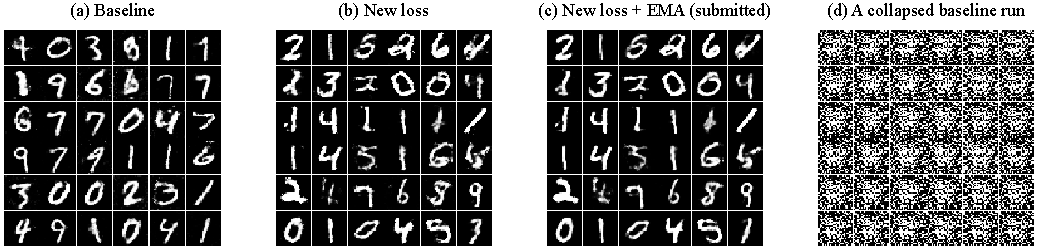
\includegraphics[width=\textwidth]{combination_samples}
\caption{\textbf{Samples from the same 36 random vectors $z$.} (a) Baseline: readable, but many ``1''s and ``7''s.
(b) New loss (Sec.~\ref{sec:training}): all digits appear. (c) Same run with averaged weights: cleaner strokes; this is the
submitted model. (d) A baseline run that collapsed: $G$ only outputs noise.}
\label{fig:samples}
\end{figure*}
